\graphicspath{{chapters/time-series/}}
Попробуем сделать то же самое, но для временных рядов. Здесь:
\begin{itemize}
	\item \textbf{Объект} --- переменная, которая меняется с течением времени
	\item \textbf{Признак} --- даты
	\item \textbf{Значение признака} --- значение переменной на конкретную дату
\end{itemize}

На Kaggle есть \href{https://www.kaggle.com/census/advance-retail-sales-time-series-collection}{выборка} по розничным продажам в различных индустриях (еда, одежда, техника и др.) в США. В ней имеются данные об объемах продаж на первое число каждого месяца, начиная с января 1992 года. Воспользуемся данной выборкой для обработки временных рядов на UMAP.

В исходных данных представлено много отраслей. Оставим только девять из них, чтобы посмотреть, как работает алгоритм. Изначально данные находятся в разных файлах --- соединим их в одну выборку.

Теперь в выборке девять объектов, представленных отраслями, но при этом 326 признаков, выраженных в количестве месяцев. То есть нам предстоит перевести 326-мерное пространство в двумерное.

Подберем гиперпараметры:
\begin{itemize}
	\item \verb|metric| --- вновь признаки объектов заданы в числовом виде $\Rightarrow$ можно использовать евклидову метрику $\Rightarrow$ \verb|metric="euclidean"| (по умолчанию)
	\item \verb|n_components| --- посмотрим на двумерное пространство $\Rightarrow$ \verb|n_components=2| (по умолчанию)
	\item \verb|min_dist| --- возьмем несколько значений \verb|min_dist|: $\{0.1, 0.3, 0.6, 1.0\}$
	\item \verb|n_neighbors| --- снова рассмотрим несколько вариантов: $\{2, 4, 5, 9\}$
\end{itemize}

Перед тем, как запускать алгоритм, необходимо обработать выборку. Данные в ней разнообразны, так как определяют продажи в разных отраслях --- соответственно, в каждой отрасли есть свой средним объем продаж, своя дисперсия. Стандартизируем выборку, что можно сделать с помощью \verb|StandardScaler| из \verb|sklearn.preprocessing|.

\newpage
Теперь можно запустить UMAP. Посмотрим, что получается:

\begin{tabular}{c|c|c|c|c}
\arrayrulecolor[rgb]{0.8,0.85,1}
	 & \verb|n_neighbors=2| & \verb|n_neighbors=3| & \verb|n_neighbors=5| & \verb|n_neighbors=7| \\
	 \hline
	 \begin{sideways} \verb|min_dist=0.1| \end{sideways} & \includegraphics*[width = 0.19\textwidth]{min=0,1,n=2.png} & \includegraphics*[width = 0.19\textwidth]{min=0,1,n=3.png} & \includegraphics*[width = 0.19\textwidth]{min=0,1,n=5.png} & 
	 \includegraphics*[width = 0.19\textwidth]{min=0,1,n=7.png} \\
	 \hline
	 \begin{sideways} \verb|min_dist=0.3| \end{sideways} & \includegraphics*[width = 0.19\textwidth]{min=0,3,n=2.png} & \includegraphics*[width = 0.19\textwidth]{min=0,3,n=3.png} & \includegraphics*[width = 0.19\textwidth]{min=0,3,n=5.png} & 
	 \includegraphics*[width = 0.19\textwidth]{min=0,3,n=7.png} \\
	 \hline
	 \begin{sideways} \verb|min_dist=0.6| \end{sideways} & \includegraphics*[width = 0.19\textwidth]{min=0,6,n=2.png} & \includegraphics*[width = 0.19\textwidth]{min=0,6,n=3.png} & \includegraphics*[width = 0.19\textwidth]{min=0,6,n=5.png} & 
	 \includegraphics*[width = 0.19\textwidth]{min=0,6,n=7.png} \\
	 \hline
	 \begin{sideways} \verb|min_dist=1.0| \end{sideways} & \includegraphics*[width = 0.19\textwidth]{min=1,0,n=2.png} & \includegraphics*[width = 0.19\textwidth]{min=1,0,n=3.png} & \includegraphics*[width = 0.19\textwidth]{min=1,0,n=5.png} & 
	 \includegraphics*[width = 0.19\textwidth]{min=1,0,n=7.png} \\
\end{tabular}
\begin{figure}[H]
	\noindent \centering {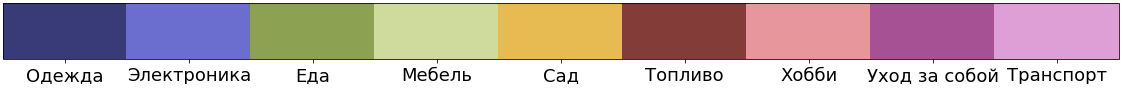
\includegraphics[width =\textwidth]{bar.png}}
\end{figure}

При маленьком значении \verb|n_neighbors| объекты собираются в кластера. Но большие значения \verb|min_dist| увеличивают расстояния между объектами, из-за чего, начиная с трех соседей, кластеры менее заметны.

При \verb|n_neighbors=5| и \verb|n_neighbors=7| кластера незаметны при любом рассмотренном значении \verb|min_dist|. Уже не видно никакой локальной структуры, только общее устройство данных.

Итак, мы получили, что при определенных значениях гиперпараметров объекты группируются в кластера. Теперь поговорим о том, зачем это нужно. В предыдущем примере кластера просто показывали разбиение по оттенкам. Для временных рядов деление на группы означает несколько другое. Кластера временных рядов показывают, какие переменные наиболее похоже по сравнению с остальными меняются во времени.
\newpage
\begin{multicols}{2}
	\fbox{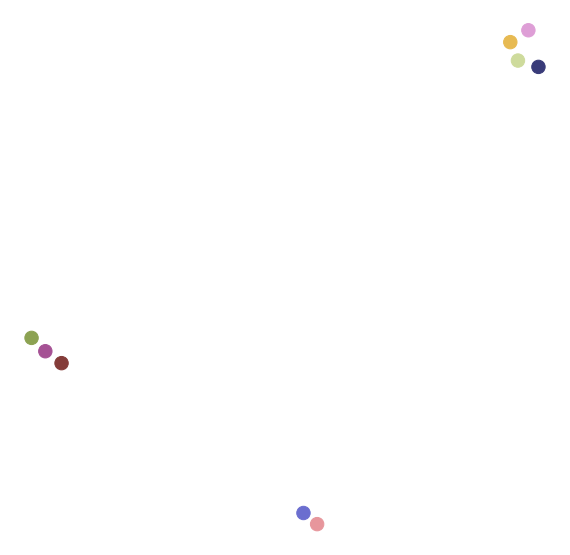
\includegraphics[width=0.9\linewidth]{show.png}\columnbreak}
	
	Рассмотрим изображение, полученное для \verb|n_neighbors=2| и \verb|min_dist=1.0|.
	
	На картинке видно три кластера. Объекты, находящиеся в каждом, похожи между собой. Так, объем розничных продаж электроники и товаров для хобби имеют сходства в траектории движения на протяжении представленных 27 лет. Аналогично можно сказать про топливо, товары для ухода за собой и еду.
	
	Если ряды в одном кластере действительно ведут себя похоже, то корреляция между ними должна быть высокой по сравнению с рядами из другого кластера.
\end{multicols}
\begin{figure}[H]
	\noindent \centering {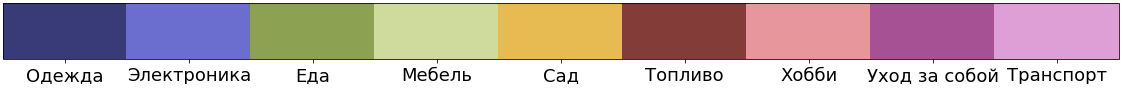
\includegraphics[width=\textwidth]{bar.png}}
\end{figure}

Посчитаем корреляцию между всеми парами объектов:
\begin{figure}[H]
	\noindent \centering {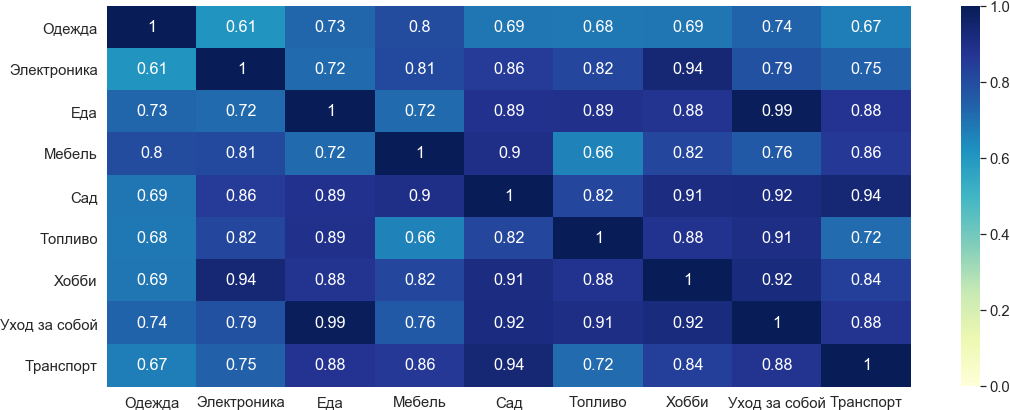
\includegraphics[width =\textwidth]{corr.png}}
\end{figure}

Рассмотрим несколько объектов и ряды, ближайшие к ним по корреляции:
\begin{itemize}
	\item \textbf{Одежда} --- мебель. И действительно, данные два объекта лежат в одном кластере, причем очень близко
	\item \textbf{Электроника} --- хобби. Аналогично, данные два ряда находятся в одном кластере, что показывает их схожесть
	\item \textbf{Мебель} --- сад. Несмотря на то, что ряд <<мебель>> был самым похожим для ряда <<одежда>>, у него самого есть ряд <<сад>> с более высоким коэффициентом корреляции. Таким образом выстраивается цепочка из соседей.
\end{itemize}

Однако UMAP меряет схожесть объектов иначе, чем коэффициент корреляции. Алгоритм учитывает относительное положение объектов, и считает похожими те, между которыми оказалось наименьшее <<расстояние>>, даже если на самом деле они находятся далеко --- просто в представленной выборке не оказалось объектов ближе. Коэффициент корреляции меряет зависимость между объектами, независимо от других объектов.

Построим график, чтобы убедиться в разнице:
\begin{figure}[H]
	\noindent \centering {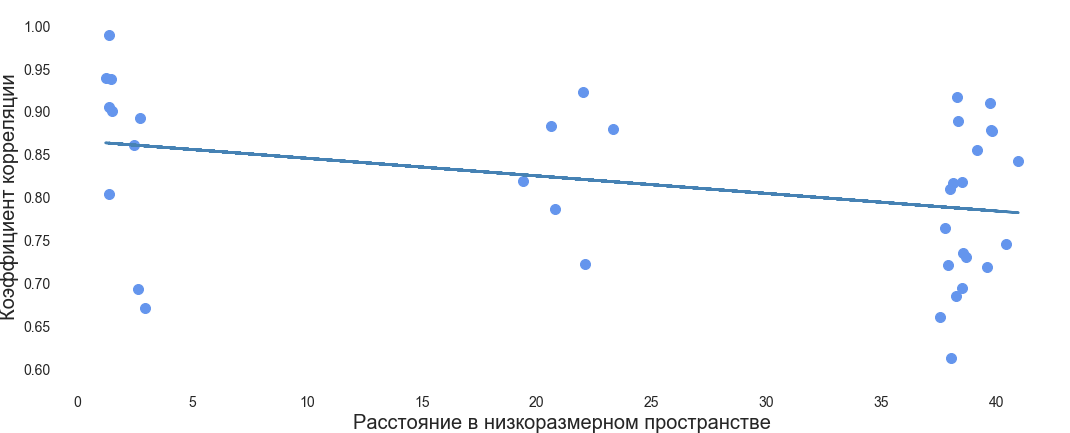
\includegraphics[width =\textwidth]{chart.png}}
\end{figure}

Каждой точке графика соответствует пара рядов. Расстояния между объектами были посчитаны\footnote{Нам не важно само значение расстояния --- нам важно далеко или близко находятся объекты}, исходя из результатов UMAP для \verb|n_neighbors=2|, \verb|min_dist=1.0|. Четкой зависимости между коэффициентом корреляции и расстоянием между объектами нет. Линия тренда показывает слабую отрицательную зависимость, что логично: чем сильнее корреляция, тем больше объекты похожи, тем меньше должно быть расстояние между ними.

Посмотрим также на подобный график для \verb|n_neighbors=7| и \verb|min_dist=1.0|. Увеличение количества соседей создает более глубокую сеть взаимосвязей между объектами, из-за чего учитываются также самые дальние соседи. Это может помочь расширить понятие схожести для UMAP, так как у него будет больше объектов для обучения.
\begin{figure}[H]
	\noindent \centering {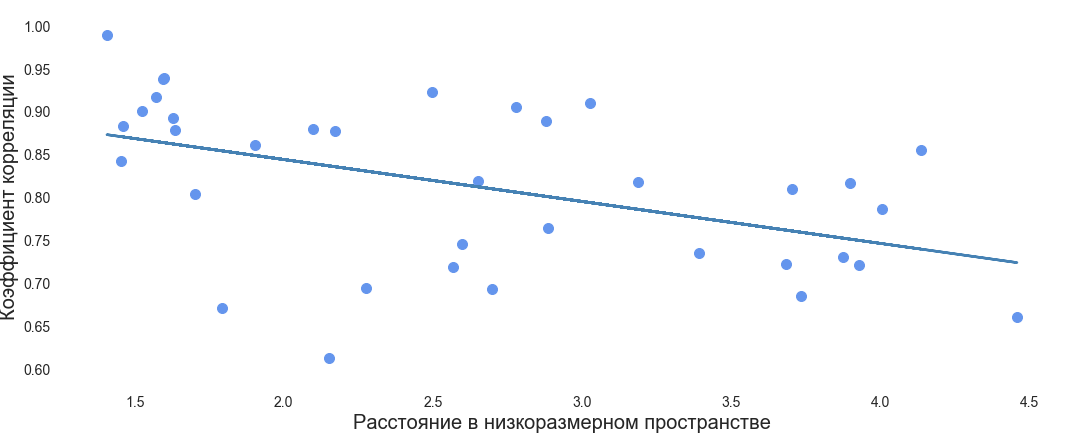
\includegraphics[width =\textwidth]{chart7.png}}
\end{figure} 

Снова линия тренда показывает отрицательную зависимость, но чуть сильнее, чем при \verb|n_neighbors=2|. Разброс точек слишком большой, чтобы говорить о четкой зависимости.

Это подтверждает приведенное ранее утверждение о различиях между данными величинами. Возможно, данная зависимость проявится при большем количестве объектов.
